\documentclass[11pt,a4paper]{article}

% ------------------------------------------------------------------ packages
\usepackage[T1]{fontenc}
\usepackage[utf8]{inputenc}
% Latin Modern (scalable) if installed; otherwise disable font expansion,
% which requires scalable fonts.
\IfFileExists{lmodern.sty}{\usepackage{lmodern}\usepackage{microtype}}%
  {\usepackage[expansion=false]{microtype}}
\usepackage[margin=2.5cm]{geometry}
\usepackage{amsmath,amssymb,amsthm}
\usepackage{booktabs}
\usepackage{tabularx}
\usepackage{enumitem}
\usepackage{xcolor}
\usepackage{graphicx}
\usepackage[section]{placeins} % floats never drift past their section
\usepackage{tikz}
\usetikzlibrary{positioning,arrows.meta,fit,shapes.geometric}
\usepackage[numbers,sort&compress]{natbib}
\usepackage[colorlinks=true,linkcolor=blue!50!black,citecolor=green!40!black,urlcolor=blue!60!black]{hyperref}
\usepackage[capitalise,noabbrev]{cleveref}

% Allow extra inter-word stretch instead of overfull lines (long \texttt names).
\setlength{\emergencystretch}{3em}

% ------------------------------------------------------------------ macros
\newcommand{\memvid}{\texttt{memvid}}
\newcommand{\cmd}[1]{\texttt{#1}}
\newcommand{\Acc}{\mathrm{Acc}}
\newcommand{\age}{\operatorname{age}}
\newcommand{\ind}{\mathbf{1}}
\newcommand{\toklen}[1]{\lvert #1 \rvert_{\tau}}
\theoremstyle{definition}
\newtheorem{definition}{Definition}

% A boxed placeholder shown until `memvid export-tex` has produced a table.
\newcommand{\pending}[1]{%
  \begin{center}\fbox{\begin{minipage}{0.85\linewidth}\small\itshape
  Pending: #1\end{minipage}}\end{center}}
% Include a generated table if it exists, otherwise show a placeholder.
\newcommand{\generated}[2]{\IfFileExists{generated/#1}{\input{generated/#1}}{\pending{#2}}}

% ------------------------------------------------------------------ title
\title{Budgeted Structured Memory for Question Answering over Long Videos\\[0.4em]
\large Course project report: \emph{Memory for long videos}}
\author{Your Name\\\small Course project: \emph{Memory for long videos}}
\date{\today}

\begin{document}
\maketitle

\begin{abstract}
A vision-language model cannot hold a long video in its context at useful
resolution, so answering questions about a 20--60 minute video requires a
memory that is written incrementally and kept within a fixed budget. We state
the problem formally and ask how the \emph{organisation} of such a memory
determines what is retained, how it is updated, how it is retrieved and
whether answers remain grounded in the source video. A frozen preprocessing
and perception pipeline turns the video into per-chunk observations; four
memory organisations (a rolling summary, a flat log, a structured memory of
entities, events, state changes and relations, and an unbounded log) consume
identical observations under identical token budgets and answer the same
questions through the same model. The analysis reports, with paired
comparisons and bootstrap intervals, what each memory keeps and loses, how
reliably it updates, whether relevant records are retrieved and cited answers
are grounded, and attributes every wrong answer of the record-based memories
to the first stage where the evidence was lost.
\end{abstract}

\tableofcontents
\bigskip

\section{Introduction and problem statement}\label{sec:intro}

\paragraph{Motivation.}
Questions about long videos are rarely answered by a single moment. ``What
colour was the board before it was painted?'' requires the system to have
noticed the board early on, to have registered the change later, and to
recognise that both observations concern the same object. ``Which tool used at
the beginning reappears at the end?'' requires linking entities across tens of
minutes. Current vision-language models (VLMs) process a bounded number of
visual tokens; a 60-minute video sampled at even one frame per second exceeds
that bound by orders of magnitude, and uniform subsampling discards exactly the
fine, transient details such questions target.

The alternative studied here is to observe the video incrementally, in short
chunks, and to maintain a \emph{memory}: a compact, queryable representation
written as the video unfolds and consulted when a question is asked. Because
the memory must itself fit into the answering model's context, it operates
under a \emph{budget}. The system must therefore decide what to store, how to
update stored knowledge when the world changes, which mentions refer to the
same entity, what to compress and what to forget.

\paragraph{Problem statement.}
Given one long video, a fixed perception pipeline that converts each chunk into
an observation, and a fixed memory budget, we ask which \emph{organisation} of
memory best supports answering questions about past events, changes of
objects, and relations between distant parts of the video, and whether the
answers it supports can be traced back to the correct source clips.

The object of study is the memory organisation, not the perception model. This
has a strict methodological consequence that shapes the whole design: every
memory variant must consume \emph{identical} per-chunk observations and operate
under the \emph{same} budget, measured in the same unit, and must be queried by
the same answering model with the same retrieval allowance. Differences in
accuracy can then be attributed to memory organisation alone. The pipeline is
therefore built in stages whose outputs are hashed and frozen before the next
stage starts, so any later deviation from them is detectable.

\paragraph{Contributions.}
\begin{enumerate}[nosep]
  \item A formal statement of budgeted incremental video memory and of the
        evaluation quantities (\cref{sec:formulation}).
  \item Four research questions derived from the project brief, each with
        operational measures (\cref{sec:rq}).
  \item A system design whose two invariants, memory-agnostic perception and
        provenance-preserving, event-sourced memory, make the planned
        comparisons valid (\cref{sec:overview}).
  \item A documented pipeline in five stages: environment check,
        video probing and reproducible preprocessing
        (\cref{sec:stage1}); a frozen evaluation set (\cref{sec:stage2});
        audited VLM perception (\cref{sec:stage3}); a structured memory with
        entity resolution, debounced state changes, compression and
        priority-based forgetting, with three baselines (\cref{sec:stage4});
        and an evaluation protocol with failure attribution, audits and an
        interactive demo (\cref{sec:stage5}).
\end{enumerate}

\section{Related work}\label{sec:related}

\paragraph{Long-video understanding.}
Benchmarks such as EgoSchema~\citep{mangalam2023egoschema},
Video-MME~\citep{fu2024videomme} and LongVideoBench~\citep{wu2024longvideobench}
show that accuracy of multimodal models degrades as videos grow longer and
that many questions require information spread over long temporal spans.
Architectural responses compress the visual token stream inside the model:
MovieChat~\citep{song2024moviechat} consolidates similar frame tokens into a
short- and long-term memory, and MA-LMM~\citep{he2024malmm} maintains a memory
bank of past visual features that is updated online. These memories are
\emph{implicit} (feature tensors) and part of a trained model; they cannot be
inspected record by record, and their contents carry no explicit timestamps.

\paragraph{Explicit memory for language agents.}
Retrieval-augmented generation~\citep{lewis2020rag} answers questions from an
external store queried at inference time. Generative
Agents~\citep{park2023generative} keep a natural-language memory stream scored
by recency, importance and relevance, and periodically write higher-level
reflections; MemGPT~\citep{packer2023memgpt} treats the context window as a
small main memory backed by external storage, with explicit operations for
moving information between the two. These systems motivate explicit,
inspectable records with salience-based eviction and summarisation, which this
project adopts, but they were designed for dialogue rather than for
perceptual streams in which the same physical object recurs and changes state.

\paragraph{Positioning.}
This project studies an \emph{explicit, structured, budgeted} memory for a
perceptual stream, with three properties not jointly present in the work
above: (i)~typed records for entities, events, state changes and relations;
(ii)~provenance from every record to source time intervals, preserved through
merging and compression, so that grounding can be measured; and (iii)~a
controlled comparison against simpler organisations under an identical budget
and identical observations. The emphasis is analytical: which information
survives, which mechanism is responsible for which gain, and where errors
originate.

\paragraph{Speech recognition.}
Transcripts are produced with Whisper~\citep{radford2023whisper} through the
CTranslate2-based faster-whisper implementation~\citep{fasterwhisper}. Whisper
is known to emit fluent but non-existent text on silence and non-speech
audio~\citep{koenecke2024careless}; the preprocessing choices
in \cref{sec:asr} are aimed at that failure mode.

\section{Problem formulation}\label{sec:formulation}

\paragraph{Video and chunks.}
Let $V$ be a video of duration $T$ seconds. It is partitioned into $n$
consecutive chunks $c_i=[u_i,v_i)$, $i=1,\dots,n$, with $u_1=0$, $v_n=T$ and
$v_i=u_{i+1}$ (the construction is given in \cref{sec:chunking}).

\paragraph{Perception.}
A fixed perception function $\phi$ maps each chunk, through its sampled frames
and the transcript segments attached to it, to an observation
$o_i=\phi(c_i)$. The function $\phi$ is \emph{memory-agnostic}: $o_i$ depends
on $c_i$ only, not on any memory state. The observations
$o_{1:n}$ are computed once and frozen.

\paragraph{Memory.}
A memory organisation is a pair $(U,R)$ of an update rule and a retrieval rule.
Starting from $M_0=\varnothing$, the update rule produces
\begin{equation}
  M_i = U(M_{i-1}, o_i), \qquad i=1,\dots,n,
\end{equation}
subject to the budget constraint
\begin{equation}\label{eq:budget}
  \toklen{M_i} \le B \quad\text{for all } i,
  \qquad \toklen{M} := \bigl|\tau\bigl(\sigma(M)\bigr)\bigr|,
\end{equation}
where $\sigma$ serialises the memory to text and $\tau$ is the tokenizer of
the answering model. Measuring the budget in answerer tokens makes it the
quantity that actually constrains answering, and makes budgets comparable
across organisations with different record formats.

\paragraph{Provenance.}
Every record $r\in M$ carries a provenance set $\pi(r)\subseteq\{1,\dots,n\}$
of the chunks it was derived from. The update rule must preserve provenance:
a record created by merging or compressing records $r_1,\dots,r_k$ receives
$\pi=\bigcup_j\pi(r_j)$. The time support of a set of records $C$ is
\begin{equation}
  I(C) = \bigcup_{r\in C}\;\bigcup_{i\in\pi(r)} [u_i,v_i).
\end{equation}

\paragraph{Answering.}
For a question $q$, the retrieval rule selects $R(q,M_n)\subseteq M_n$ with
$\toklen{R(q,M_n)}\le B_R$ (the one exception is C1, whose memory is a single
summary of size at most $B$ that is always given whole). A fixed answering model
$A$ returns an answer and the
subset of retrieved records it cites: $(\hat a,\,C)=A\bigl(q,R(q,M_n)\bigr)$,
$C\subseteq R(q,M_n)$. The answerer has no access to the video.

\paragraph{Questions.}
Each question $q$ in the evaluation set $\mathcal Q$ has a reference answer
$a^\ast(q)$, a type $\kappa(q)$ (past event, object change, cross-segment
relation, attribute recall, speech-grounded), ground-truth evidence intervals
$G(q)$, and an evidence time $e(q)$ (the latest moment needed to answer). Its
\emph{evidence age} is $\age(q)=T-e(q)$: the time elapsed between the evidence
and the end of the video, i.e.\ how long the memory had to retain it.

\paragraph{Evaluation quantities.}
For organisation $m$ at budget $B$:
\begin{align}
  y_m(q) &= \ind\bigl[\hat a \text{ is correct for } a^\ast(q)\bigr], &
  \Acc_m(B) &= \tfrac{1}{|\mathcal Q|}\textstyle\sum_{q} y_m(q),\\
  g_m(q) &= \ind\bigl[I(C)\cap G(q)\neq\varnothing\bigr], &
  \mathrm{tIoU}_m(q) &= \frac{|I(C)\cap G(q)|}{|I(C)\cup G(q)|},\\
  p_m(q) &= \frac{|I(C)\cap G(q)|}{|I(C)|}, &&
\end{align}
where $|\cdot|$ of a union of intervals is its total length and $p_m(q)=0$ when
nothing is cited. Grounding $g$ alone rewards citing records with long support
(an entity seen throughout the video overlaps every interval); the
\emph{grounding precision} $p$ and tIoU penalise it. Retrieval recall is $g$
computed with $R(q,M_n)$ in place of $C$. \emph{Evidence coverage}, used as a
proxy for fact survival, is $g$ computed with the non-entity records of $M_n$ in
place of $C$: some event, state change, relation or note derived from the
evidence chunks is still stored. It is a proxy because it shows that material
from those chunks survives, not that the specific fact does; the failure
attribution (\cref{sec:attribution}) checks the latter by hand.

\paragraph{Controlled comparison.}
The organisations compared later (\cref{tab:conditions}) differ only in
$(U,R)$. The quantities $\phi$, $o_{1:n}$, $\tau$, $B$, $B_R$ and $A$ are
shared. This is the formal content of the requirement that comparisons use
``the same observations and a similar memory budget''.

\begin{table}[ht]
\centering\small
\caption{Memory organisations to be compared (Stage~5). All share the
observations, the answerer and the retrieval allowance $B_R$.}
\label{tab:conditions}
\begin{tabularx}{\linewidth}{@{}llX@{}}
\toprule
ID & Organisation & Description \\
\midrule
C1 & Rolling summary & One text record, rewritten after each chunk under
  budget $B$; the whole summary is given to the answerer. \\
C2 & Flat log (FIFO) & One text record per observation; oldest evicted when
  over budget; embedding retrieval. \\
C3 & Structured memory & Typed records (entities, events, state changes,
  relations), entity resolution, compression, salience-based deletion;
  hybrid retrieval. \\
C4 & Unbounded flat log & C2 without eviction: an upper bound for the given
  perception. \\
\bottomrule
\end{tabularx}
\end{table}

\paragraph{A consequence for grounding.}
For C1 the memory is a single record whose provenance is every chunk seen so
far, so $I(C)$ covers most of the video and $g_{\mathrm{C1}}\approx 1$
trivially, and coverage is equally uninformative. Grounding, coverage and failure
attribution are therefore reported only for C2--C4; for C1 answer accuracy is
reported, overall, per question type and against evidence age.

\section{Research questions}\label{sec:rq}

\subsection{From the task to research questions}
The project brief asks for a memory over one long video that supports adding,
updating, merging, compressing, deleting and searching records; for questions
about past events, changes to objects, and relations between different parts
of the video; and for an analysis of what the system keeps and loses, how it
updates memory, how it finds relevant records, how accurate its answers are,
and whether its timestamps match the source clips. A comparison against a plain
text summary or another memory organisation, with the same observations and a
similar budget, is optional. \Cref{tab:task-map} shows where each requirement
is addressed.

\begin{table}[ht]
\centering\small
\caption{Requirements of the brief and where they are addressed.}\label{tab:task-map}
\begin{tabularx}{\linewidth}{@{}XX@{}}
\toprule
Requirement & Addressed by \\
\midrule
Memory structure; add, update, merge, compress, delete, search &
  structured memory C3 (\cref{sec:stage4}) \\
Questions on past events, object changes, cross-part relations &
  question types \emph{past event}, \emph{object change}, \emph{cross segment}
  (\cref{sec:stage2}) \\
What the system keeps and loses & RQ2 \\
How it updates memory after new events & RQ3 \\
How it finds relevant records & retrieval recall (RQ4) \\
Answer accuracy; timestamps vs.\ source clips & RQ1, RQ4 \\
Optional comparison, same observations and budget & baselines C1, C2, C4 (RQ1) \\
\bottomrule
\end{tabularx}
\end{table}

\subsection{Research questions}

\begin{description}[style=nextline,leftmargin=2.2em]
\item[RQ1 (accuracy and organisation).]
How accurately does the structured memory (C3) answer each type of question,
and how does it compare, at an equal budget $B$, with a rolling summary (C1),
a flat log (C2) and the unbounded log (C4)?
\item[RQ2 (what is kept and lost).]
Which information survives under a budget and which is lost first, and how
does accuracy change with evidence age $\age(q)$?
\item[RQ3 (updating).]
How reliably does the memory recognise that two mentions denote the same
entity and that an entity's attribute has changed, and how do errors in these
operations reach the answers?
\item[RQ4 (retrieval and grounding).]
Are the records relevant to a question retrieved, and do the records cited in
an answer have time support $I(C)$ overlapping the ground-truth evidence
$G(q)$?
\end{description}

\Cref{tab:rq-ops} lists how each question is measured. The analysis is
descriptive: every quantity is reported with a 95\% interval, and comparisons
between conditions are paired over questions.

\begin{table}[ht]
\centering\small
\caption{Operationalisation of the research questions.}\label{tab:rq-ops}
\begin{tabularx}{\linewidth}{@{}lXXl@{}}
\toprule
RQ & Primary measure & Secondary measures & Conditions \\
\midrule
RQ1 & $\Acc_m(B)$, overall and per question type & paired per-question
  differences (McNemar) & C1--C4, $B_1$--$B_3$ \\
RQ2 & evidence coverage (C2--C3); accuracy vs.\ $\age(q)$ (C1--C3) &
  operation-log trace of lost facts; memory size over time & C1--C3 \\
RQ3 & operation counts; merge precision and missed-merge rate (audit) &
  state-change precision; share of errors caused by corruption; ablations & C3 \\
RQ4 & retrieval recall; $g_m(q)$, $p_m(q)$, $\mathrm{tIoU}_m(q)$ & invalid citations & C2--C4 \\
\bottomrule
\end{tabularx}
\end{table}

\subsection{Expectations}
The design rests on four expectations, stated here so the reader can compare
them with the results; they are not tested as formal hypotheses.
\begin{itemize}[nosep]
\item Structured memory should help most on object-change and cross-segment
  questions, because state changes and entity identities are kept as explicit
  records that compression does not touch.
\item A rolling summary should lose fine attributes (colours, counts,
  intermediate states) before coarse events.
\item Differences between organisations should shrink as the budget grows.
\item Entity-resolution errors should be a major cause of failures on
  cross-segment questions.
\end{itemize}

\subsection{Failure attribution}\label{sec:attribution}
For each incorrect answer of a record-based organisation (C2--C4), exactly one
cause is assigned, checking the pipeline in order and stopping at the first
stage where the evidence is lost:
\begin{enumerate}[nosep]
  \item \emph{perception miss}: no observation $o_i$ with $c_i\cap G(q)\neq\varnothing$
        contains the evidence;
  \item \emph{storage loss}: it was observed but deleted or compressed away
        (traceable in the operation log);
  \item \emph{corruption}: it is stored, but a wrong merge (entity resolution)
        or a spurious state change distorted it;
  \item \emph{retrieval miss}: it is present in $M_n$ but not in $R(q,M_n)$;
  \item \emph{reasoning error}: it was retrieved, but the answer is wrong.
\end{enumerate}
The ordering makes the attribution unique and puts the burden of proof on the
earliest stage, which prevents perception errors from being misread as memory
failures.

\subsection{Statistical power and its consequences}\label{sec:power}
The planned evaluation set has 60--80 test questions. For an accuracy near
0.5 on $|\mathcal Q|=60$ questions, the half-width of a 95\% normal interval is
$1.96\sqrt{0.25/60}\approx 0.13$; for a single type with about 12 questions it
is $\approx 0.28$. Paired designs narrow these intervals considerably, because
all organisations answer the same questions, but differences below roughly
10 percentage points overall, and below 25 points within a type, cannot be
resolved. Two consequences follow. First, all comparisons are paired
(McNemar's test~\citep{mcnemar1947} for two organisations; percentile
bootstrap~\citep{efron1993bootstrap} over questions for intervals). Second,
every reported number carries a 95\% interval, and differences whose intervals
overlap substantially are described as not resolved rather than as effects.

\subsection{Threats to validity}\label{sec:threats}
\begin{itemize}[nosep]
  \item \emph{External validity}: one video, one genre. Findings concern this
        video; generalisation is argued, not measured.
  \item \emph{Perception ceiling}: all organisations inherit the errors of
        $\phi$. Its error rates are measured (Stage~3) and reported as the
        bound they impose.
  \item \emph{Annotator effects}: a single annotator writes and labels the
        questions. Mitigated by writing the questions before any memory
        exists and by tuning on the development split only.
  \item \emph{Judge bias}: free-form answers are scored with a rubric; any
        model-based judging is validated on a manually scored sample.
  \item \emph{Temporal resolution}: grounding is measured at chunk
        granularity $L$; claims about sub-chunk localisation are not possible.
\end{itemize}

\section{System overview}\label{sec:overview}

\Cref{fig:architecture} shows the complete system. Stage~1
(\cref{sec:stage1}) produces the frozen preprocessing outputs on the left;
perception (\cref{sec:stage3}) turns them into frozen observations; the
memory organisations, retrieval and answering (\cref{sec:stage4}) and the
evaluation (\cref{sec:stage5}) follow.

\begin{figure}[ht]
\centering
\resizebox{\linewidth}{!}{%
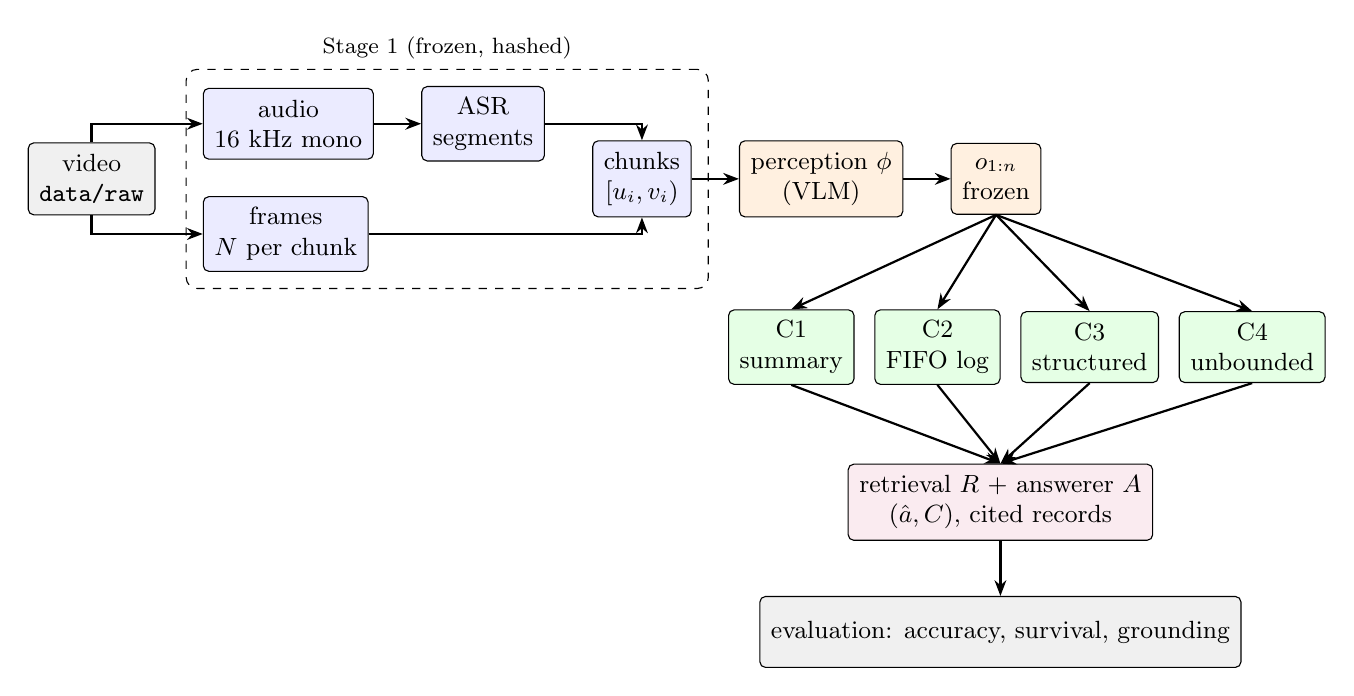
\begin{tikzpicture}[
  font=\small,
  box/.style={draw, rounded corners=2pt, align=center, minimum height=0.9cm,
              inner sep=4pt, fill=#1},
  box/.default=white,
  arr/.style={-{Stealth[length=2mm]}, thick},
  node distance=0.55cm and 0.6cm]
  \node[box=gray!12] (video) {video\\\texttt{data/raw}};
  \node[box=blue!8, right=of video, yshift=0.7cm] (audio) {audio\\16 kHz mono};
  \node[box=blue!8, right=of audio] (asr) {ASR\\segments};
  \node[box=blue!8, right=of video, yshift=-0.7cm] (frames) {frames\\$N$ per chunk};
  \node[box=blue!8, right=of asr, yshift=-0.7cm] (chunks) {chunks\\$[u_i,v_i)$};
  \node[draw, dashed, rounded corners, inner sep=6pt,
        fit=(audio)(asr)(frames)(chunks),
        label={[font=\footnotesize]above:Stage 1 (frozen, hashed)}] (s1) {};
  \node[box=orange!12, right=of chunks] (perc) {perception $\phi$\\(VLM)};
  \node[box=orange!12, right=of perc] (obs) {$o_{1:n}$\\frozen};
  \node[box=green!10, below=1.2cm of obs, xshift=-2.6cm] (c1) {C1\\summary};
  \node[box=green!10, right=0.25cm of c1] (c2) {C2\\FIFO log};
  \node[box=green!10, right=0.25cm of c2] (c3) {C3\\structured};
  \node[box=green!10, right=0.25cm of c3] (c4) {C4\\unbounded};
  \node[box=purple!8, below=1.0cm of c2, xshift=0.8cm] (ans)
       {retrieval $R$ + answerer $A$\\$(\hat a, C)$, cited records};
  \node[box=gray!12, below=0.7cm of ans] (eval)
       {evaluation: accuracy, survival, grounding};
  \draw[arr] (video) |- (audio);
  \draw[arr] (video) |- (frames);
  \draw[arr] (audio) -- (asr);
  \draw[arr] (asr) -| (chunks);
  \draw[arr] (frames) -| (chunks);
  \draw[arr] (chunks) -- (perc);
  \draw[arr] (perc) -- (obs);
  \foreach \c in {c1,c2,c3,c4} \draw[arr] (obs.south) -- (\c.north);
  \foreach \c in {c1,c2,c3,c4} \draw[arr] (\c.south) -- (ans.north);
  \draw[arr] (ans) -- (eval);
\end{tikzpicture}}
\caption{Architecture. Every memory organisation C1--C4 reads the same frozen
observations and is queried by the same retrieval allowance and answerer.}
\label{fig:architecture}
\end{figure}

\subsection{Design invariants}

\paragraph{Memory-agnostic perception.}
The perception model describes each chunk without seeing the memory. Linking a
``red mug'' in one chunk to an entity observed twenty minutes earlier is the
job of the memory, not of perception. Conditioning perception on memory would
be a natural engineering choice, since it gives the model context, but it
would make the observations depend on the organisation under test, and the
comparison of \cref{tab:conditions} would no longer be controlled.

\paragraph{Event-sourced memory.}
Every operation (insert, merge, update, compress, delete) is appended to an
operation log, and the memory after chunk $i$ is obtained by replaying the log
up to $i$. This yields three things at no extra cost: the memory-over-time view
required by the demo, an audit trail for the failure attribution of
\cref{sec:attribution}, and a correctness check (replaying the full log
reproduces the live memory exactly; this was verified for every memory
organisation during development).

\paragraph{Provenance preservation.}
The invariant of \cref{sec:formulation}, that merging and compression take the
union of provenance sets, is enforced in code and was checked after every
operation type during development. Without it, grounding (RQ4) and fact survival (RQ2) could not
be measured.

\paragraph{Single budget unit.}
The budget is measured in tokens of the answerer's tokenizer applied to the
serialised memory, for every organisation, so ``equal budget'' has one
meaning.

\subsection{Implications for Stage 1}
These invariants put four requirements on preprocessing: (i)~chunk boundaries
must be fixed once, because provenance is expressed in chunk indices;
(ii)~timestamps must be accurate and verified, because grounding compares them
with ground truth; (iii)~the inputs to perception must be byte-identical
across all later runs; (iv)~any accidental modification must be detectable.
\Cref{sec:stage1} describes how each is met.

\section{Stage 1 methodology}\label{sec:stage1}

Stage~1 consists of three steps: setting up a verifiable environment
(\cref{sec:env}), selecting the video (\cref{sec:selection}),
and preprocessing it into frozen, hashed artifacts
(\cref{sec:preprocessing}). All steps are implemented in the \memvid{} Python
package and exposed as \cmd{memvid <command>}; the commands are named in
the text. Parameter values quoted below are those of
\cmd{configs/default.yaml} and are listed in \cref{tab:stage1-params}, which is
generated from the configuration rather than copied.

\subsection{Step 1: environment and reproducibility}\label{sec:env}

\paragraph{Software.}
The package targets Python $\ge 3.10$ and uses a \cmd{src} layout with
dependencies declared in \cmd{pyproject.toml}: a small core (pydantic,
PyYAML, NumPy, Pillow, tqdm) and optional groups for speech recognition
(faster-whisper), the models (PyTorch, transformers), sentence embeddings,
figures, the demo and development tools. ffmpeg and ffprobe are system
binaries.

\paragraph{Environment check.}
\cmd{memvid check-env} records the Python and OS versions, the ffmpeg version,
the version of every relevant package, and the GPU, and fails if a hard
requirement is missing. The report is stored as JSON and exported to the
environment table below.

\paragraph{Reproducibility measures.}
\begin{enumerate}[nosep]
  \item \emph{Typed configuration.} Every run is defined by one YAML file
        validated against a schema that rejects unknown keys, so a misspelled
        parameter fails instead of silently taking its default.
  \item \emph{Determinism and freezing.} A single seed controls every random
        choice of the package (the dev/test split and the audit samples).
        Speech recognition is not fully deterministic under its default
        temperature fallback, which re-decodes difficult windows by sampling
        (configurable; disabling it gives deterministic decoding at some cost
        in quality). Identity of the inputs to later stages is therefore
        guaranteed by freezing the transcript, not by re-running ASR.
  \item \emph{Provenance manifest.} For every derived artifact the manifest
        stores its SHA-256, the producing step, a hash of the configuration
        sections that determined it, and the package version
        (\cref{sec:provenance}).
  \item \emph{Pinned versions.} The exact environment is recorded with
        \cmd{pip freeze}, and the commit used for reported results is tagged.
\end{enumerate}

\generated{environment.tex}{environment table, produced by
\cmd{memvid check-env} followed by \cmd{memvid export-tex}.}

\subsection{Step 2: video selection}\label{sec:selection}

The choice of video determines whether the research questions can be answered
at all: a video without recurring entities cannot test entity resolution, and
one without state changes cannot test updating. The video should therefore
last at least 20 minutes, as the brief requires (longer videos make evidence
age, and thus RQ2, observable over a wider range), have an audio track with
speech, contain objects and people that reappear in distant parts of the
video, and show objects whose state changes (painted, filled, assembled).

The video is placed in \cmd{data/\allowbreak raw/\allowbreak } and probed
(\cmd{memvid probe}): duration, resolution, frame rate, codecs, presence of an
audio stream, and the SHA-256 of the file, which identifies the exact source
for all later results. A video shorter than 20 minutes is reported with a
warning. The questions (Stage~2) are written before any memory exists, so they
cannot be tailored to what a particular organisation happens to capture.

\subsection{Step 3: preprocessing}\label{sec:preprocessing}

\subsubsection{Audio extraction}
The first audio stream is decoded to 16-bit PCM, mono, at 16~kHz, the native
input format of Whisper (\cmd{memvid extract-audio}). The duration of the
extracted audio is compared with the video duration; a difference above
0.5~s aborts the step, because every transcript timestamp is expressed in
audio time and would otherwise be misaligned with the frames.

\subsubsection{Speech recognition}\label{sec:asr}
Transcription uses faster-whisper~\citep{fasterwhisper} with the
\texttt{large-v3} model~\citep{radford2023whisper} and beam size~5
(\cmd{memvid transcribe}). Two settings deviate from library defaults, both
motivated by known failure modes on long recordings:
\begin{itemize}[nosep]
  \item \emph{Voice-activity filtering} (\texttt{vad\_filter=true}): non-speech
        regions are removed before decoding, which suppresses fluent but
        hallucinated text on silence and background
        sounds~\citep{koenecke2024careless}.
  \item \emph{No conditioning on previous text}
        (\texttt{condition\_on\_previous\_text=false}): with conditioning, one
        decoding error is fed back as the prompt for the next window and can
        start a repetition loop that persists for minutes.
\end{itemize}
The output is a list of segments $s_j=[a_j,b_j]$ with text, average
log-probability and no-speech probability. Segments whose no-speech
probability exceeds 0.6 are counted as suspicious and reported, not removed:
removal would be an unverified editorial decision on the evidence. Segment
timestamps are not checked by hand: transcripts enter the memory at chunk
granularity ($L=20$~s), where a boundary error of about a second changes at
most which of two adjacent chunks a segment is attached to.

\subsubsection{Chunking}\label{sec:chunking}
With chunk length $L$ and $n_0=\lfloor T/L\rfloor$, the base chunks are
$[iL,(i+1)L)$ for $i=0,\dots,n_0-1$. The remainder $r=T-n_0L$ forms an
additional chunk $[n_0L,T)$ if $r\ge\alpha L$, and is otherwise merged into
the last chunk. Hence every chunk has length in $[\alpha L,(1+\alpha)L)$
unless $T<L$. Defaults: $L=20$~s, $\alpha=0.5$ (\cmd{memvid chunk}).

The choice of $L$ is a trade-off. Smaller chunks give finer provenance, since
$L$ is the temporal resolution of every grounding result, but increase the
number of perception calls ($n\approx 180$ for one hour at $L=20$~s) and
fragment events that last longer than a chunk across several observations,
which the memory must then reassemble. A sensitivity check with
$L\in\{10,30\}$~s is planned as an ablation once perception exists.

\paragraph{Transcript assignment.}
Segment $s_j$ is attached to chunk $c_i$ iff
\begin{equation}
  \operatorname{ov}(s_j,c_i) = \min(b_j,v_i)-\max(a_j,u_i) \;\ge\;
  \min\bigl(\delta,\; b_j-a_j\bigr),
  \qquad \delta=0.25\text{ s}.
\end{equation}
The $\min$ with the segment length ensures that very short segments are
attached to the chunk containing them. A segment that straddles a boundary by
more than $\delta$ on both sides is attached to both chunks. This duplication
is deliberate: speech near a boundary is evidence for both chunks, and
assigning it to only one would make the observation of the other chunk
incomplete. A segment overlapping a chunk by less than $\delta$ is a
timestamp-noise artefact and is not attached to it.

\subsubsection{Frame sampling}
Frame $k$ of chunk $[u,v)$ is requested at the midpoint of the $k$-th of $N$
equal sub-intervals,
\begin{equation}
  t_k = u + \bigl(k+\tfrac12\bigr)\frac{v-u}{N}, \qquad k=0,\dots,N-1,
\end{equation}
(\cmd{memvid sample-frames}). Unlike endpoint sampling, midpoints never fall on
a chunk boundary, so adjacent chunks never share a frame, and the spacing
$(v-u)/N$ stays uniform across boundaries. With $N=8$ and $L=20$~s the
effective rate is $0.4$ frames/s. This rate is a real limitation and is stated
as such: a purely visual event shorter than $L/N=2.5$~s can fall between two
samples and be invisible to perception. It bounds perception recall and must
be kept in mind when interpreting perception misses
(\cref{sec:attribution}).

\paragraph{Decoding and timestamp accuracy.}
Frames are extracted by calling ffmpeg once per chunk, seeking on the input
(frame-accurate when decoding) and applying a \texttt{select} filter that keeps,
for each target $t_k$, the \emph{first frame whose presentation time is at or
after} $t_k$. The \texttt{showinfo} filter reports the true presentation time
$t_k^{\mathrm{act}}$ of each kept frame, which is stored alongside the request.
The selection rule bounds the timing error to $0\le t_k^{\mathrm{act}}-t_k<1/f$
for frame rate $f$. Frames are resized so that the longer side is at most
768~px (the visual-token cost of the VLM grows with resolution) and stored as
JPEG at quality 90.

\paragraph{Verification of the frame sampler.}
The sampler was verified on a synthetic test pattern (ffmpeg
\texttt{testsrc2}, 25~fps), in which every frame differs from every other.
Each extracted frame was compared with all frames obtained by an independent
sequential decoder (OpenCV): in every case the extracted image was
pixel-identical to the frame at the reported $t_k^{\mathrm{act}}$, and the
timing error lay in $[0,1/f)$, including targets within one frame of the end
of the stream.

\subsubsection{Provenance and freezing}\label{sec:provenance}
All artifacts of a video are written atomically (temporary file and rename)
into \cmd{data/\allowbreak derived/\allowbreak<video\_id>/} and registered in a manifest with their
hashes (\cref{app:formats}). Frames are registered as one tree hash over the
sorted pairs of relative path and file hash. After preprocessing,
\cmd{memvid freeze} verifies all hashes and marks the derived data as frozen.
From then on, any step that would overwrite a frozen artifact refuses to run
unless explicitly forced, and \cmd{memvid verify} detects any modification.
Every later stage records the manifest hash it consumed, so a result can
always be traced to the exact inputs that produced it.

\generated{stage1_params.tex}{parameter table, produced by
\cmd{memvid export-tex}.}

\subsection{Software verification}
During development the package was checked by an automated test suite (75
tests, all passing): timestamp parsing, configuration validation, chunk
construction and its edge cases, the transcript assignment rule, frame timing
and end-of-stream handling, the memory invariants (budget never exceeded,
provenance preserved, log replay reproduces the memory), scoring, and the
complete pipeline on a synthetic video. The submitted repository keeps the
smoke test instead (README), which runs every stage end to end without a GPU.

\section{Stage 1 results: data}\label{sec:stage1-results}

This section is filled automatically. After the steps of \cref{sec:stage1}
have been run on the selected video, \cmd{memvid export-tex} writes the tables
below from the manifest; until then, placeholders are shown. The numbers are
never typed by hand.

\subsection{Selected video}
\textit{Describe the selected video here: title, source and licence, genre,
duration, why it was chosen (recurring entities, state changes, speech), and
any candidates that were rejected and why.}

\subsection{Preprocessing}
\generated{stage1_results.tex}{preprocessing statistics, produced by
\cmd{memvid preprocess} and \cmd{memvid export-tex}.}

\paragraph{Checklist for interpreting the table.}
\begin{itemize}[nosep]
  \item \emph{Speech coverage} and the \emph{longest gap without speech} show
        how much of the video carries information only visually; they bound
        how useful speech-only facts can be.
  \item \emph{Suspicious segments} are candidates for hallucinated text; any
        that reach the memory should be discussed.
  \item The \emph{maximum frame timing error} must be below one frame period;
        a larger value indicates a decoding problem.
\end{itemize}

\section{Stage 2: evaluation set}\label{sec:stage2}

\paragraph{Design.}
The evaluation set consists of 60--80 questions written by hand into
\cmd{data/\allowbreak annotations/\allowbreak <video\_id>/\allowbreak questions.yaml} (template:
\cmd{templates/questions.yaml}) \emph{before any memory is built}, so the
questions cannot be shaped by what a particular organisation happens to store.
Each question carries a reference answer (and optional accepted variants), an
answer type (short text, number, yes/no, multiple choice), one of five
question types, the ground-truth evidence intervals
$G(q)$, the evidence time $e(q)$ (by default the end of the latest interval),
and the modality of the evidence. Answer types that can be scored
automatically are preferred; free text is limited to short answers. Three
question types are required by the brief: \emph{past event}, \emph{object
change} and \emph{cross segment} (relations between distant parts of the
video). Two are added to sharpen the analysis of what is lost:
\emph{attribute recall} (fine details such as counts and colours) and
\emph{speech} (facts available only in the audio).

\paragraph{Validation.}
\cmd{memvid questions-validate} rejects malformed records (unknown types,
inverted or out-of-range intervals, non-numeric answers to numeric questions,
option letters out of range, duplicate identifiers) and warns when a question
required type has fewer than eight questions, when fewer than 15\% of the questions have
evidence in the first ten minutes, or when the evidence does not cover all four
quartiles of the video. Old evidence is what tests retention (RQ2).

\paragraph{Split.}
\cmd{memvid questions-split} assigns about 15 questions to a development split
and the rest to the test split, stratified by question type with
largest-remainder allocation and a fixed seed. Thresholds, prompts and
priority weights are tuned on the development split only; the test split is
answered once, by the frozen configuration.

\paragraph{Freezing.}
\cmd{memvid questions-freeze} stores the SHA-256 of \cmd{questions.yaml} and
\cmd{split.json} in the manifest; afterwards every command that loads the
questions fails if either file changed, and re-splitting is refused.

\generated{questions_stats.tex}{question-set statistics, produced by
\cmd{memvid questions-freeze} and \cmd{memvid export-tex}.}

\section{Stage 3: perception}\label{sec:stage3}

\paragraph{Observation schema.}
For every chunk the VLM returns one JSON object with
\emph{entities} (a noun phrase with distinguishing features, a category from a
fixed list of 13, and attributes such as colour, state, count, location or
contents), \emph{events} (one present-tense sentence each, the names of the
entities involved, salience 1--3), \emph{relations} (subject, predicate,
object triples) and a \emph{speech summary}. The prompt is reproduced in
\cmd{src/\allowbreak memvid/\allowbreak prompts.py} and versioned; every cached output records the
prompt version and model.

\paragraph{Model and inputs.}
The default model is Qwen3-VL-4B-Instruct (2B when GPU memory is tight),
loaded with Hugging Face transformers or served by any OpenAI-compatible
server such as vLLM. Each call receives the $N=8$ frames of the chunk, resized
so that every frame has at most $448\times448$ pixels, and the chunk's
transcript. Resizing in our code, rather than through processor options,
makes the visual-token cost independent of the processor version. Decoding is
greedy, so outputs are reproducible for fixed inputs.

\paragraph{Validation and repair.}
The first balanced JSON object in the output is parsed and validated with
Pydantic. On failure the error and the faulty output are sent back once; a
chunk that still fails is stored as an empty observation flagged
\texttt{ok=false}, and the failure rate is reported. With the vLLM backend the
request carries the JSON schema, and decoding is constrained to it.
Normalisation lower-cases names, maps unknown categories to \emph{other},
merges duplicate names within a chunk, and drops references in events and
relations to undeclared entities (counted and reported).

\paragraph{Memory-agnostic, resumable, frozen.}
Perception never sees the memory (\cref{sec:overview}). Progress is appended
to a partial file, so an interrupted run resumes where it stopped; the final
\cmd{observations.jsonl} is hashed into the manifest and frozen with
\cmd{memvid perception-freeze}.

\paragraph{Audit.}
\cmd{memvid perception-audit} samples 20 chunks and writes a sheet with a
contact sheet of each chunk's frames. The annotator counts false entities and
missed salient events. The false-entity rate (false entities over listed
entities) must be below 15\%; together with the missed-event rate it bounds
every accuracy reported later, since all conditions inherit perception
errors.

\generated{perception_stats.tex}{perception statistics, produced by
\cmd{memvid perceive}, \cmd{memvid perception-audit-summary} and
\cmd{memvid export-tex}.}

\section{Stage 4: memory organisations}\label{sec:stage4}

All organisations write to one store that keeps the records, an append-only
operation log, an exact vector index over record texts, and the memory size
$\toklen{M}=\sum_{r\in M}|\tau(\sigma(r))|$, maintained incrementally. The
serialisation $\sigma(r)$ of a record is one line that does not depend on any
other record (names of referenced entities are copied into the record), so the
per-record counts are exact and the budget can be checked after every
operation. \Cref{tab:record-lines} shows the line formats.

\begin{table}[ht]
\centering\small
\caption{Record types and their serialisation $\sigma(r)$.}\label{tab:record-lines}
\begin{tabularx}{\linewidth}{@{}lX@{}}
\toprule
Type & Line \\
\midrule
Entity & \texttt{[E3] entity red mug (container) aka cup: color=red | seen 00:01:20-00:14:00} \\
Event & \texttt{[V12] 00:03:20-00:03:40 event: man pours water into red mug \{E1,E3\}} \\
State change & \texttt{[S4] 00:12:00 change: red mug [E3] contents: water -> empty} \\
Relation & \texttt{[R2] 00:05:00 relation: man [E1] holds drill [E5]} \\
Note (C1, C2) & \texttt{[N7] 00:02:00-00:02:20 note: <free text>} \\
\bottomrule
\end{tabularx}
\end{table}

\subsection{Structured memory (C3)}
For each observation $o_i$ the update $U$ runs five operations in order.

\paragraph{Entity resolution.}
For every observed entity $e$ and every stored entity $x$ of a compatible
category, the similarity is the largest cosine between the embedding of $e$'s
name and those of $x$'s name and aliases, minus a penalty of 0.10 when either
name is generic (``person'', ``tool'', \dots). Candidate pairs with similarity
$\ge\tau_{\mathrm{low}}=0.60$ are processed greedily in decreasing order; an
observed entity takes at most one stored entity and a stored entity is claimed
at most once per chunk (two mugs seen together are two mugs). Pairs above
$\tau_{\mathrm{high}}=0.80$ are linked; pairs in between are put to the LLM,
which sees both descriptions with their attributes and times. Unmatched
entities become new records. Every decision is logged with its similarity, for
the merge audit. Names are compared, not attributes, because attributes
legitimately change (a board is painted); the LLM sees attributes and can use
them.

\paragraph{State changes with debouncing.}
For a linked entity, an observed attribute value that differs from the stored
one opens a pending change. It is committed as a StateChange record, with time
equal to the first observation of the new value and provenance equal to the
observations that confirmed it, only after $k=2$ consecutive observations of
that entity agree. A single noisy description therefore does not create a
false change; the price is that a change is recorded one observation late.
The ablation \emph{no\_debounce} sets $k=1$.

\paragraph{Events, speech and relations.}
Events are inserted with their resolved entity identifiers. An event of the
immediately preceding chunk is extended instead when the new one has the same
entity set, a similar description (cosine $\ge0.85$) \emph{and} no content
word that the stored description lacks (a person stirring for a minute is one
event). The last condition matters: the extended event keeps its original
wording, so ``paints the board blue'' must not be merged into ``paints the
board white''. The speech summary is stored as an event of
modality \emph{speech}. Relations are deduplicated on
(subject, predicate, object).

\paragraph{Budget enforcement.}
While $\toklen{M}>B$: (i)~the oldest uncompressed events outside the three
most recent chunks are grouped into a window of 300~s and replaced by at most
three coarser events written by the LLM, with provenance equal to the union of
the originals (a window holding a single event keeps it verbatim); (ii)~when nothing is left to compress, the record with the
lowest priority is deleted,
\[
\mathrm{prio}(r)=w_{\mathrm{rec}}\,\frac{t(r)-t_{\min}}{t_{\mathrm{now}}-t_{\min}}
+\begin{cases}
w_{\mathrm{sal}}\,\mathrm{sal}(r)+w_{\mathrm{ref}}\,|\mathrm{ents}(r)| & \text{event}\\
w_{\mathrm{sal}}+2w_{\mathrm{ref}} & \text{relation}\\
2w_{\mathrm{sal}}+w_{\mathrm{sc}} & \text{state change}\\
w_{\mathrm{ent}}+w_{\mathrm{ref}}\cdot\#\text{references} & \text{entity}
\end{cases}
\]
with $(w_{\mathrm{sal}},w_{\mathrm{ref}},w_{\mathrm{rec}},w_{\mathrm{sc}},w_{\mathrm{ent}})=(1,0.5,1,2,3)$.
Entities and state changes are never compressed: they are compact and carry
exactly the facts that object-change and cross-segment questions ask for
(the first expectation in \cref{sec:rq}).

\subsection{Baselines}
\begin{description}[nosep]
\item[C1 rolling summary.] After each chunk the LLM rewrites one summary from
  the previous summary and the new observation, under a word limit derived
  from $B$; the result is cut to the longest word prefix whose line fits $B$
  exactly. The answerer receives the whole summary.
\item[C2 flat log.] One note per observation (its text serialisation);
  the oldest note is evicted while $\toklen{M}>B$.
\item[C4 unbounded log.] C2 without eviction: the upper bound for this
  perception. Its final size defines the budgets: $B_k=f_k\cdot\toklen{M_{\mathrm{C4}}}$
  with $f=(0.02,0.05,0.15)$.
\end{description}
The ablations of C3 switch off entity resolution, state changes, compression,
or debouncing, one at a time.

\subsection{Retrieval and answering}\label{sec:retrieval}
For C2--C4, the score of a record is its cosine similarity to the question,
plus 0.25 when it is, or refers to, an entity whose name occurs in the
question, plus $0.20\,w_t$ for temporal cues: \emph{beginning/first} favours
early records, \emph{end/last} late ones, and \emph{after X}/\emph{before X}
favours records just after/before the best match for X with weight
$\exp(-\text{gap}/300\,\mathrm{s})$. The top 40 records are taken in score
order while they fit $B_R=1500$ tokens, and presented in temporal order. The
answerer returns an answer, the identifiers of the supporting records, and a
confidence; citations of records it was not shown are discarded and counted.
The time support of the cited records is the predicted evidence $I(C)$.

\section{Stage 5: evaluation protocol}\label{sec:stage5}

\paragraph{Runs.}
\cmd{memvid run-all} builds C4, resolves the budgets, then builds and answers
C1--C3 at $B_1$--$B_3$ and the four C3 ablations at $B_2$ (14 runs). It
refuses to run on unfrozen questions or observations. Each run stores its
final records, the full operation log, the resolution log, the size trace,
the models and a signature of its inputs. A run whose configuration, models,
observations or budget changed is rebuilt automatically, and answers are redone
when the memory, the questions or the retrieval settings change, so a result
can never come from stale inputs.

\paragraph{Scoring.}\label{sec:scoring}
Numbers are parsed (digits or number words) and compared with 5\% relative
tolerance (timestamps in the answer are ignored); yes/no is compared after
parsing; for multiple choice the option text is matched before a bare letter,
so ``a drill'' is not read as option A. Short text is correct on normalised exact
match, or when every content word of a reference answer is contained in the
answer and the answer is neither negated nor a list of alternatives (at most
$\max(2,|r|)$ extra content words for a reference of $|r|$ words). Remaining short-text answers go to the LLM judge
(\cref{sec:threats}), whose verdicts are cached and validated on all judged
items in a manual audit; manual scores override the judge.

\paragraph{Failure attribution and audits.}
For every wrong answer of C2--C4 the code proposes the first stage where the
evidence was lost (\cref{sec:attribution}): no record overlapping $G(q)$
survives (storage loss, with the operations that removed them), an
overlapping record involves a merge or a state change judged wrong in the
audits (corruption), nothing overlapping was retrieved (retrieval miss), or
the answer is wrong despite retrieval (reasoning error). The annotator
confirms each proposal and marks perception misses from the observations.
The merge audit labels 50 links and 50 new-entity
decisions of C3 at $B_2$ (merge precision and missed-merge rate); the state
audit labels 30 detected changes (precision). All rates carry Wilson
intervals.

\paragraph{Statistics.}
All comparisons are paired over questions: exact McNemar tests for two
conditions on the same questions, and 95\% percentile bootstrap intervals with
$10^4$ resamples of questions for every accuracy and rate. Audit rates carry
Wilson intervals.

\paragraph{Demo.}
\cmd{memvid demo} starts a Gradio application with three views: memory over
time (a slider replays the operation log to any chunk and shows the records,
the operations of that chunk and a timeline), question answering on the final
memory of any run with the retrieved and cited records and the supporting clip
(cut with ffmpeg), and the same question answered by every condition side by
side.

\paragraph{Scope relative to the brief.}
Everything the brief requires is implemented (\cref{tab:task-map}). Beyond it,
the project adds two question types (attribute recall and speech), three
budget levels, ablations of the structured memory, manual audits and a failure
attribution, all of which deepen the analysis of what is kept and lost and how
memory is updated. Exact vector search is used instead of an approximate index:
with at most a few thousand records it is fast and has no approximation error.

\section{Results}\label{sec:results}

All tables and figures in this section are produced by \cmd{memvid analyze}
from the run outputs; none is typed by hand. Until the analysis has been run,
placeholders are shown.

\newcommand{\genfig}[3]{\IfFileExists{figures/#1.pdf}{%
  \begin{figure}[ht]\centering\includegraphics[width=#2\linewidth]{figures/#1.pdf}%
  \caption{#3}\label{fig:#1}\end{figure}}{\pending{figure \texttt{\detokenize{#1}} (produced by \cmd{memvid analyze})}}}

\subsection{Accuracy and organisation (RQ1)}
\generated{results_accuracy.tex}{accuracy table}
\genfig{accuracy_vs_budget}{0.7}{Accuracy against the memory budget; the band is the 95\% interval of the unbounded log C4.}
\generated{results_by_type.tex}{accuracy by question type}
\genfig{accuracy_by_type}{0.8}{Accuracy by question type at the ablation budget.}
\generated{results_mcnemar.tex}{paired comparisons}

\subsection{What is kept and lost (RQ2)}
\genfig{retention}{0.7}{Accuracy against evidence age (quartiles of age).}
\genfig{memory_size}{0.7}{Memory size over the video; the dashed line is the budget.}

\subsection{Updating, retrieval and grounding (RQ3, RQ4)}
\generated{results_operations.tex}{operation counts per run}
\generated{results_grounding.tex}{survival, retrieval and grounding}
\generated{results_ablations.tex}{ablations}
\generated{audit_stats.tex}{audit results}

\subsection{Where answers fail}
\generated{results_attribution.tex}{failure attribution}
\genfig{attribution}{0.8}{Wrong answers by the first stage where the evidence was lost.}

\paragraph{Case studies.}
\textit{Trace one success and two failures through the operation log (the demo
shows the operations per chunk): where the evidence entered the memory, which
operation changed or removed it, and what the answerer saw.}

\section{Limitations and conclusions}\label{sec:conclusion}

\paragraph{Limitations.}
\begin{itemize}[nosep]
\item One video of one genre: the findings describe this video.
\item Every condition inherits the perception errors measured in
      \cref{sec:stage3}; accuracy is bounded by them.
\item One annotator wrote the questions and the audit labels; agreement
      between annotators is not measured.
\item Entity resolution compares names only (and LLM judgements in the
      ambiguous band); visual re-identification was not used.
\item Grounding is measured at chunk granularity ($L=20$~s).
\end{itemize}

\paragraph{Conclusions.}
\textit{Answer RQ1--RQ4 in turn from \cref{sec:results}: how accurate the
structured memory is and where it beats the baselines, what is lost first under
a budget, how reliable updating is, whether relevant records are retrieved and
answers stay grounded; then compare with the expectations of \cref{sec:rq}.}


\bibliographystyle{plainnat}
\bibliography{references}

\appendix
\section{Data formats}\label{app:formats}

\subsection{Derived artifacts}
Machine-generated, stored in \cmd{data/\allowbreak derived/\allowbreak <video\_id>/\allowbreak }. Times are in
seconds from the start of the video.

\begin{table}[ht]
\centering\small
\begin{tabularx}{\linewidth}{@{}lX@{}}
\toprule
File & Content (one JSON object per line for \texttt{.jsonl}) \\
\midrule
\texttt{video\_info.json} & duration, resolution, frame rate, codecs, audio
  stream, SHA-256 of the source \\
\texttt{audio.wav} & 16 kHz mono 16-bit PCM \\
\texttt{transcript.jsonl} & \texttt{segment\_id, start, end, text,
  avg\_logprob, no\_speech\_prob} \\
\texttt{asr\_info.json} & model, device, compute type, detected language,
  wall time, real-time factor, settings \\
\texttt{chunks.jsonl} & \texttt{chunk\_id, t\_start, t\_end,
  transcript\_text, segment\_ids} \\
\texttt{frames/index.jsonl} & \texttt{chunk\_id, frame\_index, t\_target,
  t\_actual, path, width, height} \\
\texttt{frames/chunk\_XXXX/fYY.jpg} & resized frames \\
\texttt{manifest.json} & per artifact: path, SHA-256 (tree hash for frames),
  size, producing step, configuration hash, package version, time; statistics
  per step; frozen stages \\
\bottomrule
\end{tabularx}
\end{table}


\end{document}
